\documentclass{beamer}
\usetheme{}
\usecolortheme{dolphin}           
\useinnertheme{circles}
\setbeamertemplate{itemize items}[default]
\setbeamertemplate{enumerate items}[default]
\usepackage[T1]{fontenc}
\usepackage[utf8]{inputenc}
\usepackage{lmodern}
\usepackage{amsmath}
\usepackage{booktabs} 
\usepackage{graphicx}        
\usepackage{array}
\usepackage{color}
\makeatletter
\def\zapcolorreset{\let\reset@color\relax\ignorespaces}
\def\colorrows#1{\noalign{\aftergroup\zapcolorreset#1}\ignorespaces}
\makeatother
\graphicspath{{/home/swl/Dropbox/ucd/advanced_macro/figures/}} 
\setbeamertemplate{navigation symbols}{}
\setbeamertemplate{footline}[frame number]

%--------------------------------------
\title{New Keynesian model}
\author{School of Economics, University College Dublin}
\date{Spring 2018}
\begin{document}

%--------------------------------------
\begin{frame}
 \titlepage
\end{frame}
%--------------------------------------

%--------------------------------------
\begin{frame}
  Kydland \& Prescott (1982) "Time to Build and Aggregate Fluctuations" showed strength of DSGE modeling
  \begin{itemize}
    \item Small coherent model of economy
    \item Optimising agents, rational expectations, market clearing
    \item Model generated data that resembled observed data
  \end{itemize}
  \medskip
  Some shortcomings
  \begin{itemize}
    \item Volatility of hours, persistence of output    
  \end{itemize}
  \medskip
  But model did remarkably well excluding a lot of presumed \textit{sine qua nons}
  \begin{itemize}
    \item Money, nominal rigidities (i.e. stickiness), non-market clearing
  \end{itemize}
\end{frame}
%--------------------------------------

%--------------------------------------
\begin{frame}
  \textbf{Q:} Does money matter?
\end{frame}
%--------------------------------------

%--------------------------------------
\begin{frame}
  Short-term fluctuations linked to money increase through price stickiness 
  \begin{itemize}
    \item Hume, Keynes, Friedman
  \end{itemize}
  \medskip
  Strong empirical case supporting notion that money matters
  \begin{itemize}
    \item "A Monetary History of the U.S.", Friedman \& Schwartz (1971)
    \item Empirical evidence from VAR models
  \end{itemize}
\end{frame}
%--------------------------------------

%--------------------------------------
\begin{frame}
  Can include money into DSGE model, requires
  \begin{enumerate}
    \item Monopolistic competition
    \item Role to justify existence of money (e.g. in utility)
    \item Monetary authority inducing nominal shocks to economy
  \end{enumerate}
  \medskip
  Model fit improves by
  \begin{enumerate}
    \item Delay/extend response economy to shock (e.g. habit persistence)
    \item Adding extra shocks (e.g. preferences)
  \end{enumerate}
\end{frame}
%--------------------------------------


%--------------------------------------
\begin{frame}
  \textbf{New Keynesian model} addresses some of critiques on Keynesian model
  \begin{itemize}
    \item Rational expectations
    \item People behave optimally
  \end{itemize}
  \medskip
  Room for systematic effects of monetary policy  
  \begin{itemize}
    \item Central mechanism for monetary policy is \textbf{sticky prices}
    \item If prices don't move in line with money; central bank can't control real money supply or interest rate
  \end{itemize}
\end{frame}
%--------------------------------------


%--------------------------------------
\begin{frame}
  Basic features of NK model
  \begin{itemize}
    \item General equilibrium model
    \item Two stages of production: firms are monopolistically competitive
    \item Firms cannot reoptimise prices each period
    \item Due to price stickiness monetary policy has real effects: needs to be described by model
  \end{itemize}
  \medskip
  Basically NK model is RBC model with
  \begin{enumerate}
    \item Sticky prices
    \item Monetary authority operating via interest rate feedback rule
    \item Additional simplifications
    \begin{itemize}
      \item No capital accumulation (only labour); no trend productivity growth, only stationary shocks 
    \end{itemize}
  \end{enumerate}
\end{frame}
%--------------------------------------

%--------------------------------------
\begin{frame}
  Why are prices sticky?
  \begin{itemize}
    \item Imperfect information
    \item Costs of changing prices
    \item Agents trust in price stability (in stable economic environment)
  \end{itemize}
\end{frame}
%--------------------------------------


%--------------------------------------
\begin{frame}
 To describe optimal behaviour, use \textbf{Dixit-Stiglitz model}\\
\begin{align}
  Y_t=\left( \int_0^1 Y_t(i)^{\frac{\theta-1}{\theta}}di\right)^{\frac{\theta}{\theta-1}}
\end{align}
Consumers maximise utility function $U(Y_t)$ over an aggregate of a continuum of differentiated goods
\begin{itemize}
  \item $\theta$ denotes constant elasticity of substitution
\end{itemize}
\medskip
 Model only includes consumption goods, no capital
\end{frame}
%--------------------------------------


%--------------------------------------
\begin{frame}
 For each differentiated good, demand function has form 
\begin{align}
  Y_t(i)=Y_t \left( \frac{P_t(i)}{P_t}\right)^{-\theta}
\end{align}
\medskip
$P_t$ is the aggregate price index which is defined by
\begin{align}
  P_t=\left( \int_o^1 P_t(i)^{1-\theta}di \right)^{\frac{1}{1-\theta}}
\end{align}  
\end{frame}
%--------------------------------------

%--------------------------------------
\begin{frame}
 To describe price rigidity use \textbf{Calvo model}\\ 
\begin{align}
  P_t &= \left[(1-\alpha)X_t^{1-\theta} + \alpha P_{t-1}^{1-\theta} \right] ^{\frac{1}{1-\theta}}\\ \nonumber
  P_t^{1-\theta} &= (1-\alpha)X_t^{1-\theta} + \alpha P_{t-1}^{1-\theta}
\end{align}
\end{frame}
%--------------------------------------

%--------------------------------------
\begin{frame}
Random fraction of firms is able to reset prices
\begin{align}
   1-\alpha 
\end{align}
Firms reset price to 
\begin{align}
   X_t 
\end{align}
\begin{enumerate}
  \item All other firms keep prices unchaged
  \item All firms setting new prices today set the same price.
\end{enumerate}
\medskip
 Firms are completely symmetric: except for timing of price-setting
\end{frame}
%--------------------------------------

%--------------------------------------
\begin{frame}
 Prices may be fixed for many periods: firms pick price to maximise
\begin{align}
  \mathbb{E}_t \left[ \sum_{k=0}^{\infty} (\alpha \beta)^k (Y_{t+k}P_{t+k}^{\theta-1}X_t^{1-\theta} -
  P_{t+k}^{-1}C (Y_{t+k}P_{t+k}^{\theta}X_t^{-\theta}) ) \right]
\end{align}
$C(.)$ is the cost function\\
Differentiate with respect to $X_t$ to get solution of maximisation problem
\begin{align}
  X_t = \frac{\theta}{\theta-1} \frac{\mathbb{E}_t \left(\sum_{k=0}^{\infty}(\alpha \beta)^k Y_{t+k}P_{t+k}^{\theta-1}MC_{t+k} \right)}
  {\mathbb{E}_t \left(\sum_{k=0}^{\infty}(\alpha \beta)^k Y_{t+k}P_{t+k}^{\theta-1} \right) }
\end{align}  
\end{frame}
%--------------------------------------

%--------------------------------------
\begin{frame}
  \begin{align*}
  X_t = \frac{\theta}{\theta-1} \frac{\mathbb{E}_t \left(\sum_{k=0}^{\infty}(\alpha \beta)^k Y_{t+k}P_{t+k}^{\theta-1}MC_{t+k} \right)}
  {\mathbb{E}_t \left(\sum_{k=0}^{\infty}(\alpha \beta)^k Y_{t+k}P_{t+k}^{\theta-1} \right) }
  \end{align*}
  \medskip
  Without pricing frictions, firm sets
  \begin{align}
    X_t=\frac{\theta}{\theta-1}MC_t
  \end{align}
  \medskip
  i.e. price is markup over marginal costs  \\
  Price likely to be fixed for number of periods
  \begin{itemize}
    \item Optimal price is markup over weighted average of future marginal costs
  \end{itemize}
\end{frame}
%--------------------------------------

%--------------------------------------
\begin{frame} 
  \begin{align}    (\alpha \beta)^k  \end{align}
    Less weight on future MC because of 
    \begin{enumerate}[i]
      \item Discounting
      \item Lower probability for price set at $t$ to be around at $k$ as $k$ increases
    \end{enumerate}
    \begin{align} Y_{t+k}P_{t+k}^{\theta-1}   \end{align}
    Represents aggregate factors affecting future firm demand
    \begin{enumerate}[i]
      \item $Y_{t+k}$ increases firm will sell more; as $P_{t+k}$ goes up, firm's relative price down and demand increases
      \item Will offset discounting term (somewhat)
    \end{enumerate}
\end{frame}
%--------------------------------------

%--------------------------------------
\begin{frame}
  Have two non-linear equations for price
\begin{align}
    P_t^{1-\theta} &= (1-\alpha)X_t^{1-\theta} + \alpha P_{t-1}^{1-\theta}\\
    X_t &= \frac{\theta}{\theta-1} \frac{\mathbb{E}_t \left(\sum_{k=0}^{\infty}(\alpha \beta)^k Y_{t+k}P{t+k}^{\theta-1}MC_{t+k} \right)}
  {\mathbb{E}_t \left(\sum_{k=0}^{\infty}(\alpha \beta)^k Y_{t+k}P{t+k}^{\theta-1} \right) }
\end{align}
\medskip
  Not easy to solve or simulate price equation
  \begin{itemize}
    \item  Use log-linear approximations taken around constant growth, zero inflation path
  \end{itemize}
\end{frame}
%--------------------------------------

%--------------------------------------
\begin{frame}  
  Zero-inflation steady-state is such that  
    \begin{align}
    X_t^* &= P_t^*=P^*_{t-1}=P^*\\  
  \end{align}
  \begin{align}
    P_t^{1-\theta} &= (1-\alpha)X_t^{1-\theta} + \alpha P_{t-1}^{1-\theta}
  \end{align}
  Becomes
  \begin{align}
    (P^*)^{1-\theta} (1+(1-\theta)p_t)=& (1-\alpha)(P^*)^{1-\theta} (1+(1-\theta)x_t)+ \\ \nonumber
    &\alpha(P^*)^{1-\theta}(1+(1-\theta)p_{t-1})
  \end{align}
  Simplifies to
  \begin{align}
    p_t=(1-\alpha)x_t+\alpha p_{t-1}
  \end{align}
\end{frame}
%--------------------------------------

%--------------------------------------
\begin{frame} 
 FOC for optimal pricing is given by
 \begin{align}
   \mathbb{E}_t \left [ \sum_{k=0}^{\infty} (\alpha \beta)^k \left( (1-\theta)Y_{t+k}P_{t+k}^{\theta-1}X_t^{-\theta} + \theta MC_{t+k}Y_{t+k}P_{t+k}^{\theta-1}X_t^{-\theta-1} \right)\right]=0
 \end{align}
 Around steady-state we get
 \begin{align}
   (1-\theta)Y_{t+k}P_{t+k}^{\theta-1}X_t^{-\theta} & \approx  (1-\theta)Y^*(P^*)^{\theta-1}(X^*)^{-\theta} \\ \nonumber 
   &(1+y_{t+k}+(\theta-1)p_{t+k}-\theta x_t)\\
  \theta MC_{t+k}Y_{t+k}P_{t+k}^{\theta-1}X_t^{-\theta-1} & \approx \\ \nonumber 
  & \theta MC^* Y^* (P^*)^{\theta-1} (X^*)^{-\theta-1} \\ \nonumber &(1+mc_{t+k} + y_{t+k} + (\theta -1) p_{t+k} - (1-\theta) x_t)
 \end{align}
\end{frame}
%--------------------------------------

%--------------------------------------
\begin{frame}
  Can use that in steady-state 
  \begin{align}
    X^* = \left( \frac{\theta}{\theta-1}\right ) MC^*
  \end{align}
  Simplifies to
  \begin{align}
    \mathbb{E}_t \left[ \sum_{k=0}^{\infty} (\alpha \beta)^k (x_t - mc_{t+k}) \right] &=0 \\ \nonumber  
    x_t &= (1-\alpha \beta) \sum_{k=0}^{\infty} (\alpha \beta)^k \mathbb{E}_t mc_{t+k}
  \end{align}
  Aggregate output and price level drop out: log-price is weighted average of expected future logs  of marginal costs
\end{frame}
%--------------------------------------

%--------------------------------------
\begin{frame}
  Calvo model pricing dynamics can be summarised by
  \begin{align*}
    p_t&=(1-\alpha)x_t+\alpha p_{t-1} \\
    x_t &= (1-\alpha \beta) \sum_{k=0}^{\infty} (\alpha \beta)^k \mathbb{E}_t mc_{t+k}
  \end{align*}
  \begin{itemize}
    \item $p_t$ can be solved using Binder-Pesaran method
    \item $x_t$ has infinite sum: describes standard solution to first-order stochastic difference equation
  \end{itemize}
\end{frame}
%--------------------------------------


%--------------------------------------
\begin{frame}
  Reverse engineering 
  \begin{align}
    x_t &= (1-\alpha \beta) \sum_{k=0}^{\infty} (\alpha \beta)^k \mathbb{E}_t mc_{t+k}
  \end{align}
  can write optimal reset price as
  \begin{align}
  x_t=(1-\alpha \beta) mc_t + (\alpha \beta) \mathbb{E}_t x_{t+1}
 \end{align}
 Can combine this with fact that 
\begin{align}
  p_t &= (1-\alpha)x_t+\alpha p_{t-1}\\ \nonumber
  \frac{1}{1-\alpha}(p_t-\alpha p_{t-1}) &= x_t 
\end{align}
\end{frame}
%--------------------------------------

%--------------------------------------
\begin{frame}
  \textbf{Inflation rate} given by
  \begin{align}
    \pi_t=p_t-p_{t-1}
  \end{align}
  After bunch of re-arranging you get  
\begin{align}
  \pi_t= \beta \mathbb{E}_t \pi_{t+1} + \frac{(1+\alpha)(1-\alpha \beta)}{\alpha}(mc_t - p_t)
\end{align}
$\pi_t$ is a function 
\begin{enumerate}
  \item Expected inflation in $t+1$
  \item Real marginal cost
\end{enumerate}
  This is the \textbf{New-Keynesian Phillips curve} (NKPC)
\end{frame}
%--------------------------------------

%--------------------------------------
\begin{frame}
  \textbf{Output}\\
  Assume diminishing returns to labour production function
  \begin{itemize}
    \item Higher output reduces marginal productivity and raises marginal cost 
  \end{itemize}
  \medskip
  Makes real marginal costs a function of output gap  
\begin{align}
  mc_t-p_t=\eta x_t
\end{align}
Concerning $x_t$
\begin{align}
  x_t=y_t-y_t^n
\end{align}
$y_t^n$ is output path in zero-inflation price friction free economy
\end{frame}
%--------------------------------------

%--------------------------------------
\begin{frame}
 NKPC has form
  \begin{align}
  \pi_t=\beta \mathbb{E}_t \pi_{t+1} + \kappa x_t
\end{align}
\medskip
 Looks like traditional expectations-augmented Phillips curve.\\
 First-order stochastic difference equation; has solution in form
\begin{align}  
  \pi_t=\kappa \sum_{k=0}^{\infty}\beta^k \mathbb{E}_t x_{t+k} 
\end{align}
\end{frame}
%--------------------------------------

%--------------------------------------
\begin{frame}
 No backward-looking element in
\begin{align}  
  \pi_t=\kappa \sum_{k=0}^{\infty}\beta^k \mathbb{E}_t x_{t+k} 
\end{align}
\begin{itemize}
  \item No intrinsic inertia in inflation
  \item Lagged inflation effects statistical artifacts in conventional models
\end{itemize}
\medskip
Original NKPC formulation has no shock/error term
\begin{itemize}
  \item Maybe price movements not consistent with this formulation.
\end{itemize}
\begin{align}
  \pi_t=\beta \mathbb{E}_t \pi_{t+1} + \kappa x_t + u_t
\end{align} 
\medskip
Can add \textbf{cost-push shock} NKPC  
\end{frame}
%--------------------------------------

%--------------------------------------
\begin{frame}
  \begin{align}
  \pi_t=\beta \mathbb{E}_t \pi_{t+1} + \kappa x_t + u_t
\end{align} 
 $u_t$ accounts for misc. shocks:
 \begin{itemize}
   \item $\pi$ no longer results of just expected inflation and output gap
 \end{itemize}
 \medskip
 Central bank can no longer implement a stabilisation policy by only addressing the output gap. 
\end{frame}
%--------------------------------------

%--------------------------------------
\begin{frame}
  NKPC links inflation to output
  \begin{itemize}
    \item Need to consider how to link output to monetary policy
  \end{itemize}
  \medskip  
  NK model uses interest rates: recall exclusion of capital in model
  \begin{align}
    Y=C
  \end{align}
   Relation between $C$ and $i$ comes from standard intertemporal optimization problem; consumer wants to maximise
\begin{align}  
 \sum_{k=0}^{\infty}\left(\frac{1}{1+\beta}\right)^k U(C_{t+k}) 
 \end{align}  
\end{frame}
%--------------------------------------

%--------------------------------------
\begin{frame}
  Intertemporal budget constraint given by  
\begin{align}
  \sum_{k=0}^{\infty} \frac{\mathbb{E}_t C_{t+k}}{\left(\prod_{m=1}^{k+t}R_{t+m} \right)} =
   A_t +   \sum_{k=0}^{\infty} \frac{\mathbb{E}_t Y_{t+k}}{\left(\prod_{m=1}^{k+t}R_{t+m} \right)}
\end{align}
$R_t$ is the interest rate\\
Can write Lagrangian as
\begin{align}
  \mathcal{L} &= \sum_{k=0}^{\infty} \left(\frac{1}{1+\beta} \right)^k U(C_{t+k}) \\ \nonumber
  &+ \lambda \left[A_t + \sum_{k=0}^{\infty} \frac{\mathbb{E}_t Y_{t+k}}{\left( \prod_{m=1}^{k+1} R_{t+m} \right)} -
  \sum_{k=0}^{\infty} \frac{\mathbb{E}_t C_{t+k}}{\left( \prod_{m=1}^{k+1} R_{t+m} \right)} \right ]
\end{align}
\end{frame}
%--------------------------------------

%--------------------------------------
\begin{frame}
  Derive \textbf{Euler equation} by combining FOCs for $C_t$ and $C_{t+1}$ 
\begin{align}  
  U'(C_t) = \mathbb{E}_t \left[ \left(\frac{R_{t+1}}{1+\beta} \right) U'(C_{t+1})\right] 
  \end{align}
  Can set
  \begin{align}
    U(C_t)=U(Y_t)=\frac{Y_t^{1-\frac{1}{\sigma}}}{1-\frac{1}{\sigma}}
  \end{align}
  \begin{align}
  \mathbb{E}_t \left[ \left( \frac{R_{t+1}}{1+\beta} \right) \left( \frac{Y_t}{Y_{t+1}} \right)^{\frac{1}{\sigma}} \right]=1 
 \end{align}
 Similar to the Real Business Cycle model this is a Constant Relative Risk Aversion (CRRA) utility from consumption
\end{frame}
%--------------------------------------

%--------------------------------------
\begin{frame}
  Set 
  \begin{align}
    \rho=-log\beta
  \end{align}
Log-linearised version of the Euler equation is 
\begin{align}  
y_t=\mathbb{E}_ty_{t+1} - \sigma(i_t - \mathbb{E}_t\pi_{t+1} - \rho) 
\end{align}
i.e. today's output depends negatively on the real interest rate
\end{frame}
%--------------------------------------


%--------------------------------------
\begin{frame}
  Recall that inflation equation featured output gap  
  \begin{align}
    x_t=y_t-y_t^n  
  \end{align}
  Can rewrite Euler equation as
\begin{align}
  x_t &= \mathbb{E}_t x_{t+1} - \sigma (i_t - \mathbb{E}_t \pi_{t+1} - \rho) + \mathbb{E}_t y_{t+1}^n - y_t^n\\  
\end{align}
\medskip
More naturally this becomes
\begin{align}
  x_t &= \mathbb{E}_t x_{t+1} - \sigma (i_t - \mathbb{E}_t \pi_{t+1} - r_t^n) \\ 
  r_t^n&=\sigma^{-1}\mathbb{E}_t\Delta y_{t+1}^n - log \beta  
\end{align}
\end{frame}
%--------------------------------------

%--------------------------------------
\begin{frame}
  This defines a 'natural' real interest rate $r_t$ which is consistent with
  \begin{align}
    x_t=\mathbb{E}_tx_{t+1}
  \end{align}
  and a function of   
  \begin{align}
    \mathbb{E}_t \Delta y_{t+1}^n
  \end{align}
  \medskip
  Meaning that it is determined by 
  \begin{enumerate}
    \item Technology
    \item Preferences
  \end{enumerate}
  Output gap $x_t$ follows a first-order stochastic difference equation which has a solution of the form
\begin{align}
  x_t = \sigma \sum_{k=0}^{\infty} (i_{t+k} - \mathbb{E}_t \pi_{t+k+1} - r_{t+k}^n)  
\end{align}  
\end{frame}
%--------------------------------------

%--------------------------------------
\begin{frame}
  \textbf{Policy implications}\\
  No backward-looking elements in $x_t$
  \begin{itemize}
    \item Output has no intrinsic persistence
  \end{itemize}
  \medskip
  Implication for monetary policy is that what matters for today's output is
   \begin{enumerate}
     \item Current policy
     \item All future interest rates
   \end{enumerate}
\end{frame}
%--------------------------------------

%--------------------------------------
\begin{frame}
  Central bankers should therefore take care in managing expectations about future policy
  \begin{itemize}
    \item Future interest rates are their key tool
  \end{itemize}
Interpreting $i_t$ as the short-term interest rate, and assuming that the expectations theory of the term structure holds, this model states that it is the long-term interest rates that matter for spending.   
\end{frame}
%--------------------------------------


%--------------------------------------
\begin{frame}
  In most basic form NK model has three equations
\begin{enumerate}
  \item New Keynesian Phillips curve
  \begin{align} \pi_t=\beta \mathbb{E}_t \pi_{t+1} + \kappa x_t + u_t \end{align}
  \item Euler equation for output
  \begin{align} x_t = \mathbb{E}_t x_{t+1} - \sigma (i_t - \mathbb{E}_t \pi_{t+1} - r_t^n) \end{align}
\end{enumerate}
 \medskip
 Only need one final equation: description of how interest rate policy is set.
\end{frame}
%--------------------------------------

%--------------------------------------
\begin{frame}
  \textbf{Output-inflation dynamics}
\begin{align}
  x_t &=\mathbb{E}_tx_{t+1} - \sigma(i_t-\mathbb{E}_t\pi_{t+1} - r_t^n)\\
  \pi_t &= \beta \mathbb{E}_t \pi_{t+1} + \kappa x_t + u_t
\end{align}
\medskip
Can rewrite as  
\begin{align}
  \pi_t = \beta \mathbb{E}_t \pi_{t+1} + \kappa \mathbb{E}_t x_{t+1} - \kappa\sigma(i_t - \mathbb{E}_t \pi_{t+1} - r_t^n) + u_t
\end{align}
 Put in vector form
\begin{align}
  \begin{pmatrix} x_t \\ \pi_t \end{pmatrix} = \begin{pmatrix} 1 & \sigma \\ \kappa & \beta +\kappa\sigma \end{pmatrix}
  \begin{pmatrix} \mathbb{E}_tx_{t+1} \\ \mathbb{E}_t \pi{t+1} \end{pmatrix} + 
  \begin{pmatrix} \sigma (r_t^n-i_t) \\ \kappa\sigma (r_t^n-i_t) + u_t \end{pmatrix}
\end{align}  
\end{frame}
%--------------------------------------

%--------------------------------------
\begin{frame}
 Have model in form
 \begin{align}
  Z_t=A\mathbb{E}_tZ_{t+1}+BV_t 
 \end{align}
 \medskip
 Unique stable solution requires eigenvalues $A$ to be less than 1
\begin{align} 
 A=\begin{pmatrix} 1 & \sigma \\ \kappa & \beta +\kappa\sigma \end{pmatrix} 
 \end{align}
 Recall that there is an eigenvector that when multiplied by $A-\lambda I$ equals a vector of zeroes, meaning that the determinants of the matrix equal zero
\end{frame}
%--------------------------------------

%--------------------------------------
\begin{frame}
  \begin{align}
  A-\lambda I = \begin{pmatrix}
    1-\lambda & \sigma \\
    \kappa    & \beta + \kappa \sigma - \lambda
  \end{pmatrix}
 \end{align}
 Eigenvalues satisfy
\begin{align} 
    P(\lambda) &=(1-\lambda)(\beta+\kappa\sigma-\lambda)-\kappa\sigma=0\\ \nonumber
    P(\lambda) &= \lambda^2  -(1+\beta+\kappa\sigma)\lambda+\beta=0
\end{align} 
\end{frame}
%--------------------------------------

%--------------------------------------
\begin{frame} $P(\lambda)$ is a U-shaped polynomial, we have that
 \begin{align}
   P(0)&=\beta>0\\
   P(1)&=-\kappa \sigma <0
 \end{align}
 $P(\lambda)>0$ when $\lambda>1$; this implies
 \begin{enumerate}
   \item one eigenvalue between zero and one 
   \item one eigenvalue greater than 1
 \end{enumerate}
\medskip
Serious problem for the model: no unique stable solution; model has multiple equilibria
\end{frame}
%--------------------------------------

%--------------------------------------
\begin{frame}
  Two options to deal with $\lambda$ issue
\begin{enumerate}
  \item Accept multiple equilibria: analyse impact interest rate changes on output and inflation across range of different possible equilibria
  \item Specify monetary policy following a particular rule; rule designed to produce a unique stable equilibrium
\end{enumerate}
\end{frame}
%--------------------------------------

%--------------------------------------
\begin{frame}
  \textbf{Taylor rule}  
\begin{align} 
  i_t=r_t^n+ \phi_{\pi}\pi_t+\phi_xx_t 
\end{align}
 \medskip
  Interest rate based on inflation and output gap
  \begin{itemize}
    \item Increase in $\pi,x$ will increase $i$    
  \end{itemize}
  \medskip
 Note inclusion of natural interest rate: set interest rate moves with the natural interest rate
 \begin{itemize}
   \item Rule here allows $i$ to move with natural rate: Taylor's rule has a constant intercept
 \end{itemize}
\end{frame}
%--------------------------------------

%--------------------------------------
\begin{frame}
  Rule can be substituted in the equation for $x_t$ to give
\begin{align}  
  x_t=\mathbb{E}_tx_{t+1} + \sigma \mathbb{E}_t \pi_{t+1} - \sigma\phi_{\pi}\pi_t -\sigma\phi_x x_t 
\end{align}  
 To look at dynamics rewrite equations in matrix form
 \begin{align}
  Z_t&=\begin{pmatrix} x_t \\ \pi_t \end{pmatrix}; V_t=\begin{pmatrix}  0 \\u_t \end{pmatrix} \\
  Z_t&=A\mathbb{E}_tZ_{t+1}+BV_t 
 \end{align}
\end{frame}
%--------------------------------------


%--------------------------------------
\begin{frame}
 In standard model
 \begin{align*}
   Z_t=A\mathbb{E}_tZ_{t+1}+BV_t 
 \end{align*}
  We have
  \begin{align}
  A &= \frac{1}{1+\sigma\pi_x + \kappa\sigma\phi_{\pi}} \begin{pmatrix}
    1 & \sigma(1-\beta\phi_{\pi}) \\
    \kappa & \beta + \sigma\kappa + \beta(1+\sigma\phi_x)
      \end{pmatrix}\\
  B &= \frac{1}{1+\sigma\phi_x + \kappa\sigma\phi_{\pi}} \begin{pmatrix}
    1 & -\sigma\phi_{\pi}\\
    \kappa & 1+\sigma\phi_x
  \end{pmatrix}
\end{align}  
\end{frame}
%--------------------------------------

%--------------------------------------
\begin{frame}
  System is a matrix version of the first-order stochastic difference equation: can be solved in a similar fashion to give
\begin{align}
  Z_t=\sum_{k=0}^{\infty}A^k B\mathbb{E}_tV_{t+k}
\end{align}
 For unique stable equilibrium absolute values of both eigenvalues of $A$ need to be less than 1, which will be the case when
\begin{align}  
  \phi_{\pi}+\frac{(1-\beta)\phi_x}{\kappa}>1 
\end{align}
$\beta \approx 1$ so the condition is approximately $\phi_{\pi}>1$
\end{frame}
%--------------------------------------

%--------------------------------------
\begin{frame}
  If the policy rule satisfies this requirement, known as the \textbf{Taylor principle}, there is a unique stable equilibrium
  \begin{itemize}
    \item Nominal interest rates must rise by more than inflation so that real rates rise in response to an increase in inflation
    \item Needed for stability because otherwise inflationary shocks reduces real interest rates which stimulates the economy which will further stimulate inflation
  \end{itemize}
  \medskip
  A big question for central banks of course is what is optimal to do? 
  In general we know that central banks 
\begin{itemize}
  \item Don't like inflation 
  \item Like to keep output on a steady path close to potential output
\end{itemize}
\end{frame}
%--------------------------------------

%--------------------------------------
\begin{frame}  
   Central bank behaviour can be modeled using \textbf{loss function}
  \begin{align} 
  L_t = \frac{1}{2}\sum_{t=0}^{\infty}\beta^t\mathbb{E}_t(\pi_{t+k}^2 + \gamma x_{t+k}^2) 
\end{align}
$x_t$ is the output gap\\
$\gamma$ weight put on output stabilisation relative to inflation stabilisation\\
\medskip
Research has shown that 
 \begin{align}
   \gamma=\frac{\kappa}{\theta}   
 \end{align}
 $\kappa$ is coefficient on output gap in NKPC\\
 $\theta$ is elasticity of demand for firms 
\end{frame}
%--------------------------------------

%--------------------------------------
\begin{frame}
  \begin{align*}
    x_t^2 
  \end{align*}
  Risk-averse consumers prefer smooth consumption paths which keeps output close to its natural rate to achieve this.
  \begin{align*}
    \pi_t^2
  \end{align*}
  Consumers don't just care about the level of consumption but also its allocation. 
  \begin{itemize}
    \item With inflation, sticky prices imply different prices for symmetric goods and thus different consumption levels
    \item Optimality requires equal consumption of all items in the bundle; rationale for welfare effect of inflation, independent of its effect on output
  \end{itemize}
\end{frame}
%--------------------------------------

%--------------------------------------
\begin{frame}
  Central bank has two options in setting policy
  \begin{enumerate}
    \item Under commitment: solves problem at beginning of time
    \item Under discretion: solves problem each period
  \end{enumerate}
\end{frame}
%--------------------------------------

%--------------------------------------
\begin{frame}
  \textbf{Optimal policy under commitment}\\
  Suppose that the central bank can commit today to a strategy it can adopt now and in the future. 
\begin{align}
  \mathcal{L}= \sum_{t=0}^{\infty} \beta^t \mathbb{E}_t \left[ -\frac{1}{2} (\pi_{t+k}^2 + \gamma x_{t+k}^2) + 
  \lambda_{t+k} (\pi_{t+k} - \beta \pi_{t+k+1} - \kappa x_{t+k}) \right] 
\end{align}
FOCs are 
\begin{align}
  \frac{\partial \mathcal{L}}{\partial x_t} &= \gamma \mathbb{E}_t x_{t+k} - \kappa \mathbb{E}_t \lambda_{t+k} &= 0\\
  \frac{\partial \mathcal{L}}{\partial \pi_t} &=\mathbb{E}_t\pi_{t+k} + \mathbb{E}_t\lambda_{t+k} - \mathbb{E}_t \lambda_{t+k-1} &=0
\end{align}
for $t=0,1,2,...$ where $\lambda_{-1}=0$
\begin{itemize}
  \item There is no constraint on time $t=-1$
\end{itemize}
\end{frame}
%--------------------------------------

%--------------------------------------
\begin{frame}
  Can re-arrange terms
\begin{align}
  \mathbb{E}_t x_{t+k} &= \frac{\kappa}{\gamma} \mathbb{E}_t\lambda_{t+k} = \theta \mathbb{E}_t \lambda_{t+k} \\
  \mathbb{E}_t \pi_{t+k} &= \mathbb{E}_t \lambda_{t+k-1} - \mathbb{E}_t \lambda_{t+k} = -\frac{1}{\theta}\mathbb{E}_t \Delta x_{t+k}\\
  \Delta \mathbb{E}_t x_{t+k} &= - \theta \mathbb{E}_t \pi_{t+k}
\end{align}
\medskip
Optimal policy \textbf{under commitment} is therefore characterised by
\begin{align}
  x_t &= -\theta\pi_t = \theta(p_{t-1}-p_t)\\
  \mathbb{E}_t \Delta x_{t+1} &= -\theta \mathbb{E}_t \pi_{t+k} = \theta (p_{t+k-1} - p_{t+k})
\end{align}  
\end{frame}
%--------------------------------------

%--------------------------------------
\begin{frame}
  Considering initial price level  $p_{-1}$ we get
\begin{align}  
  \mathbb{E}_t x_{t+k} = \theta(p_{-1} - \mathbb{E}_tp_{t+k}) 
\end{align}
\medskip
Since
\begin{align}
  \pi_t=p_t-p_{t-1}
\end{align}
\medskip
Price level targeting rule
\begin{itemize}
  \item Implies that price level always returns to trend
  \item Inflation will be zero, on average
\end{itemize}
\end{frame}
%--------------------------------------


%--------------------------------------
\begin{frame}
  \textbf{Optimal policy under discretion}\\  \medskip
  Consider scenario where a central bank cannot commit to taking a particular course of action in the future
  \begin{itemize}
    \item Can only set optimal strategy for what to do today    
  \end{itemize}
  \medskip
  Optimality conditions for period $t$ is
\begin{align}
  x_t &= -\theta\pi_t
\end{align}
 \medskip
 "Lean against the wind" policy
 \begin{itemize}
   \item $x_t>0$: pursue policy that lowers inflation
 \end{itemize}
\end{frame}
%--------------------------------------

%--------------------------------------
\begin{frame}
 Under optimal discretionary policy, policy is set against inflation
\begin{align}
  \pi_t=\beta \mathbb{E}_t\pi_{t+1}-\kappa\theta\pi_t+u_t
\end{align}
\medskip
First-order difference equation
\begin{align}
  \pi_t=\left(\frac{1}{1+\theta\kappa}\right) (\beta \mathbb{E}_t\pi_{t+1} + u_t)
\end{align}
\medskip
Repeated iteration solution
\begin{align}
  \pi_t = \left(\frac{1}{1+\theta\kappa}\right) \sum_{k=0}^{\infty} \left(\frac{\beta}{1+\theta\kappa}\right)^k \mathbb{E}_tu_{t+k}
\end{align}
\end{frame}
%--------------------------------------

%--------------------------------------
\begin{frame}
  \textbf{Cost-push} shocks assumed to follow $AR(1)$ process, implying
  \begin{align}
    \mathbb{E}_tu_{t+k}=\rho^ku_t
  \end{align}
  \medskip
  With 
  \begin{align}
 u_t&=\rho u_{t-1} + v_t \\ \nonumber v_t &\sim N(0,\sigma^2) 
\end{align}
\end{frame}
%--------------------------------------

%--------------------------------------
\begin{frame}
  Using
  \begin{align}
    \sum_{k=0}^{\infty}c^k=\frac{1}{1-c}
  \end{align}
for $|c|<1$, inflation becomes
\begin{align}
  \pi_t &= \left( \frac{1}{1-\theta\kappa} \right) \left[ \sum_{k=0}^{\infty} \left( \frac{\beta\rho}{1+\theta\kappa} \right)^k \right]u_t\\
  &= \left( \frac{1}{1-\theta\kappa} \right) \left( \frac{1}{1-\frac{\beta\rho}{1+\theta\kappa}} \right) u_t\\
  &= \frac{u_t}{1+\theta\kappa-\beta\rho}
\end{align}
\end{frame}
%--------------------------------------%--------------------------------------
\begin{frame}
  $AR(1)$ cost-push shock implies that 
\begin{align}
  \mathbb{E}_tx_{t+1} &= \rho x_t\\
  \mathbb{E}_t \pi_{t+1} &= \rho \pi_t  
\end{align}
\medskip
Substitute into Euler equation along with
\begin{align}
  x_t&=-\theta\pi_t\\ \nonumber
  x_t&=\mathbb{E}_t x_{t+1}-\sigma(i_t-\mathbb{E}_t \pi_{t+1}-r_t^n)
\end{align}
\medskip
to back out what the optimal interest rate looks like  
\end{frame}
%--------------------------------------

%--------------------------------------
\begin{frame}
  \begin{align}
  i_t=r_t^n+ \left( \rho + \frac{(1-\rho)\theta}{\sigma} \right) \pi_t
\end{align}
\medskip
This will be greater than 1 if 
\begin{align}
 \frac{\theta}{\sigma}>1 
\end{align}
\medskip
 which will hold for all reasonable parameterisations
\begin{itemize}
   \item Inflation and interest rates do not depend at all on what happened in the past.
 \end{itemize} 
\end{frame}
%--------------------------------------

%--------------------------------------
\begin{frame}
  \textbf{Woodford} (2003) argues that policy under commitment produces superior welfare outcomes
  \begin{itemize}
    \item Private sector will anticipate future policies will be different
    \item Conditions at time $t$ have the potential to improve stabilisation outcomes at time $t+1$
    \item Holds even if these conditions will actually no longer matter at a later time. 
  \end{itemize}
\end{frame}
%--------------------------------------

%--------------------------------------
\begin{frame}
  Have to consider the transitory cost-push shock $u_t$; Woodford argues expectations about shock won't affect future policy
  \begin{itemize}
    \item Short-run trade-off between inflation and the output gap; shift vertically by
    \begin{align}
       u_t
     \end{align} 
    \item Central bank has to choose whether to increase inflation, have a negative output gap, or possibly a bit of both
  \end{itemize}
  Due to shocks people can expect central bank to pursue tighter policy from $t+1$ onwards;short-run trade-off will be shifted by the change 
  \begin{align}
   u_t+\mathbb{E}_t\pi_{t+1} 
  \end{align}
  Shift will actually be smaller and thus possibly increase stabilisation: main issue is that it might not be practically feasible to pick a policy and stick to it.   
\end{frame}
%--------------------------------------

%--------------------------------------
\begin{frame}
  \textbf{Empirical issues}\\ \medskip
  Central role for NKPC in NK model: relies on output gap $x_t$
  \begin{itemize}
    \item How to measure this gap?
  \end{itemize}
  \medskip
  Can assume that on average output tend to return to its natural rate
 \begin{itemize}
   \item Use simple trend as proxy for natural rate (e.g. HP-filter)
 \end{itemize}
\end{frame}
%--------------------------------------

%--------------------------------------
\begin{frame}
 Proxy
 \begin{align}
  x=y_t-y_t^n
 \end{align}
 with
\begin{align}
  \tilde{x}_t=y_t-\hat{y}_t
\end{align}
\medskip
Can estimate NKPC using 
\begin{align}
  \pi_t = \beta \mathbb{E}_t \pi_{t+1} + \kappa\tilde{x}_t
\end{align}
\medskip
Cannot observe $\mathbb{E}_t \pi_{t+1}$: substitute realised $\pi_{t+1}$ 
\begin{itemize}
  \item Use an instrumental variable to deal with the fact this this is a noisy estimator of what we really want.
\end{itemize}
\end{frame}
%--------------------------------------

%--------------------------------------
\begin{frame} 
  For model
  \begin{align*}
    \pi_t = \beta \mathbb{E}_t\pi_{t+1} + \kappa \tilde{x}_t
  \end{align*}
  results often show 
  \begin{align*}
    \kappa<0
  \end{align*}  
\end{frame}
%--------------------------------------

%--------------------------------------
\begin{frame}
Seems counterintuitive but we know that
\begin{enumerate}
  \item $\Delta\pi_t$ is negatively correlated with the unemployment rate
  \item Therefore positively correlated with the output gap
\end{enumerate}
\medskip
  Given that $\beta\approx1$, we can proxy
\begin{align}
  \pi_t-\beta \mathbb{E}_t\pi_{t+1}
\end{align} 
with 
\begin{align}
  \pi_t-\pi_{t+1}=-\Delta\pi_{t+1}
\end{align}
Negative sign on $\kappa$ might not be that surprising: two possible reasons for failure
\begin{enumerate}
  \item Model is wrong
  \item Output gap measured with error
\end{enumerate}
\end{frame}
%--------------------------------------


%--------------------------------------
\begin{frame}
  \textbf{Gali \& Gertler} (1999) argue output gap is measured with error
  \begin{itemize}
    \item Deterministic trends do a bad job in capturing movements in the natural rate of output
  \end{itemize}
  \medskip
  Suggest using unit labour costs as proxy for marginal costs
  \begin{itemize}
    \item Proxy for real marginal costs is the labour share of income.
  \end{itemize}
  Estimate 
  \begin{align}
   \pi_t = \beta \mathbb{E}_t \pi_{t+1} + \gamma s_t    
  \end{align}
  Find
  \begin{align}
    \beta>0
  \end{align} 
\end{frame}
%--------------------------------------

%--------------------------------------
\begin{frame}
  \begin{figure}
    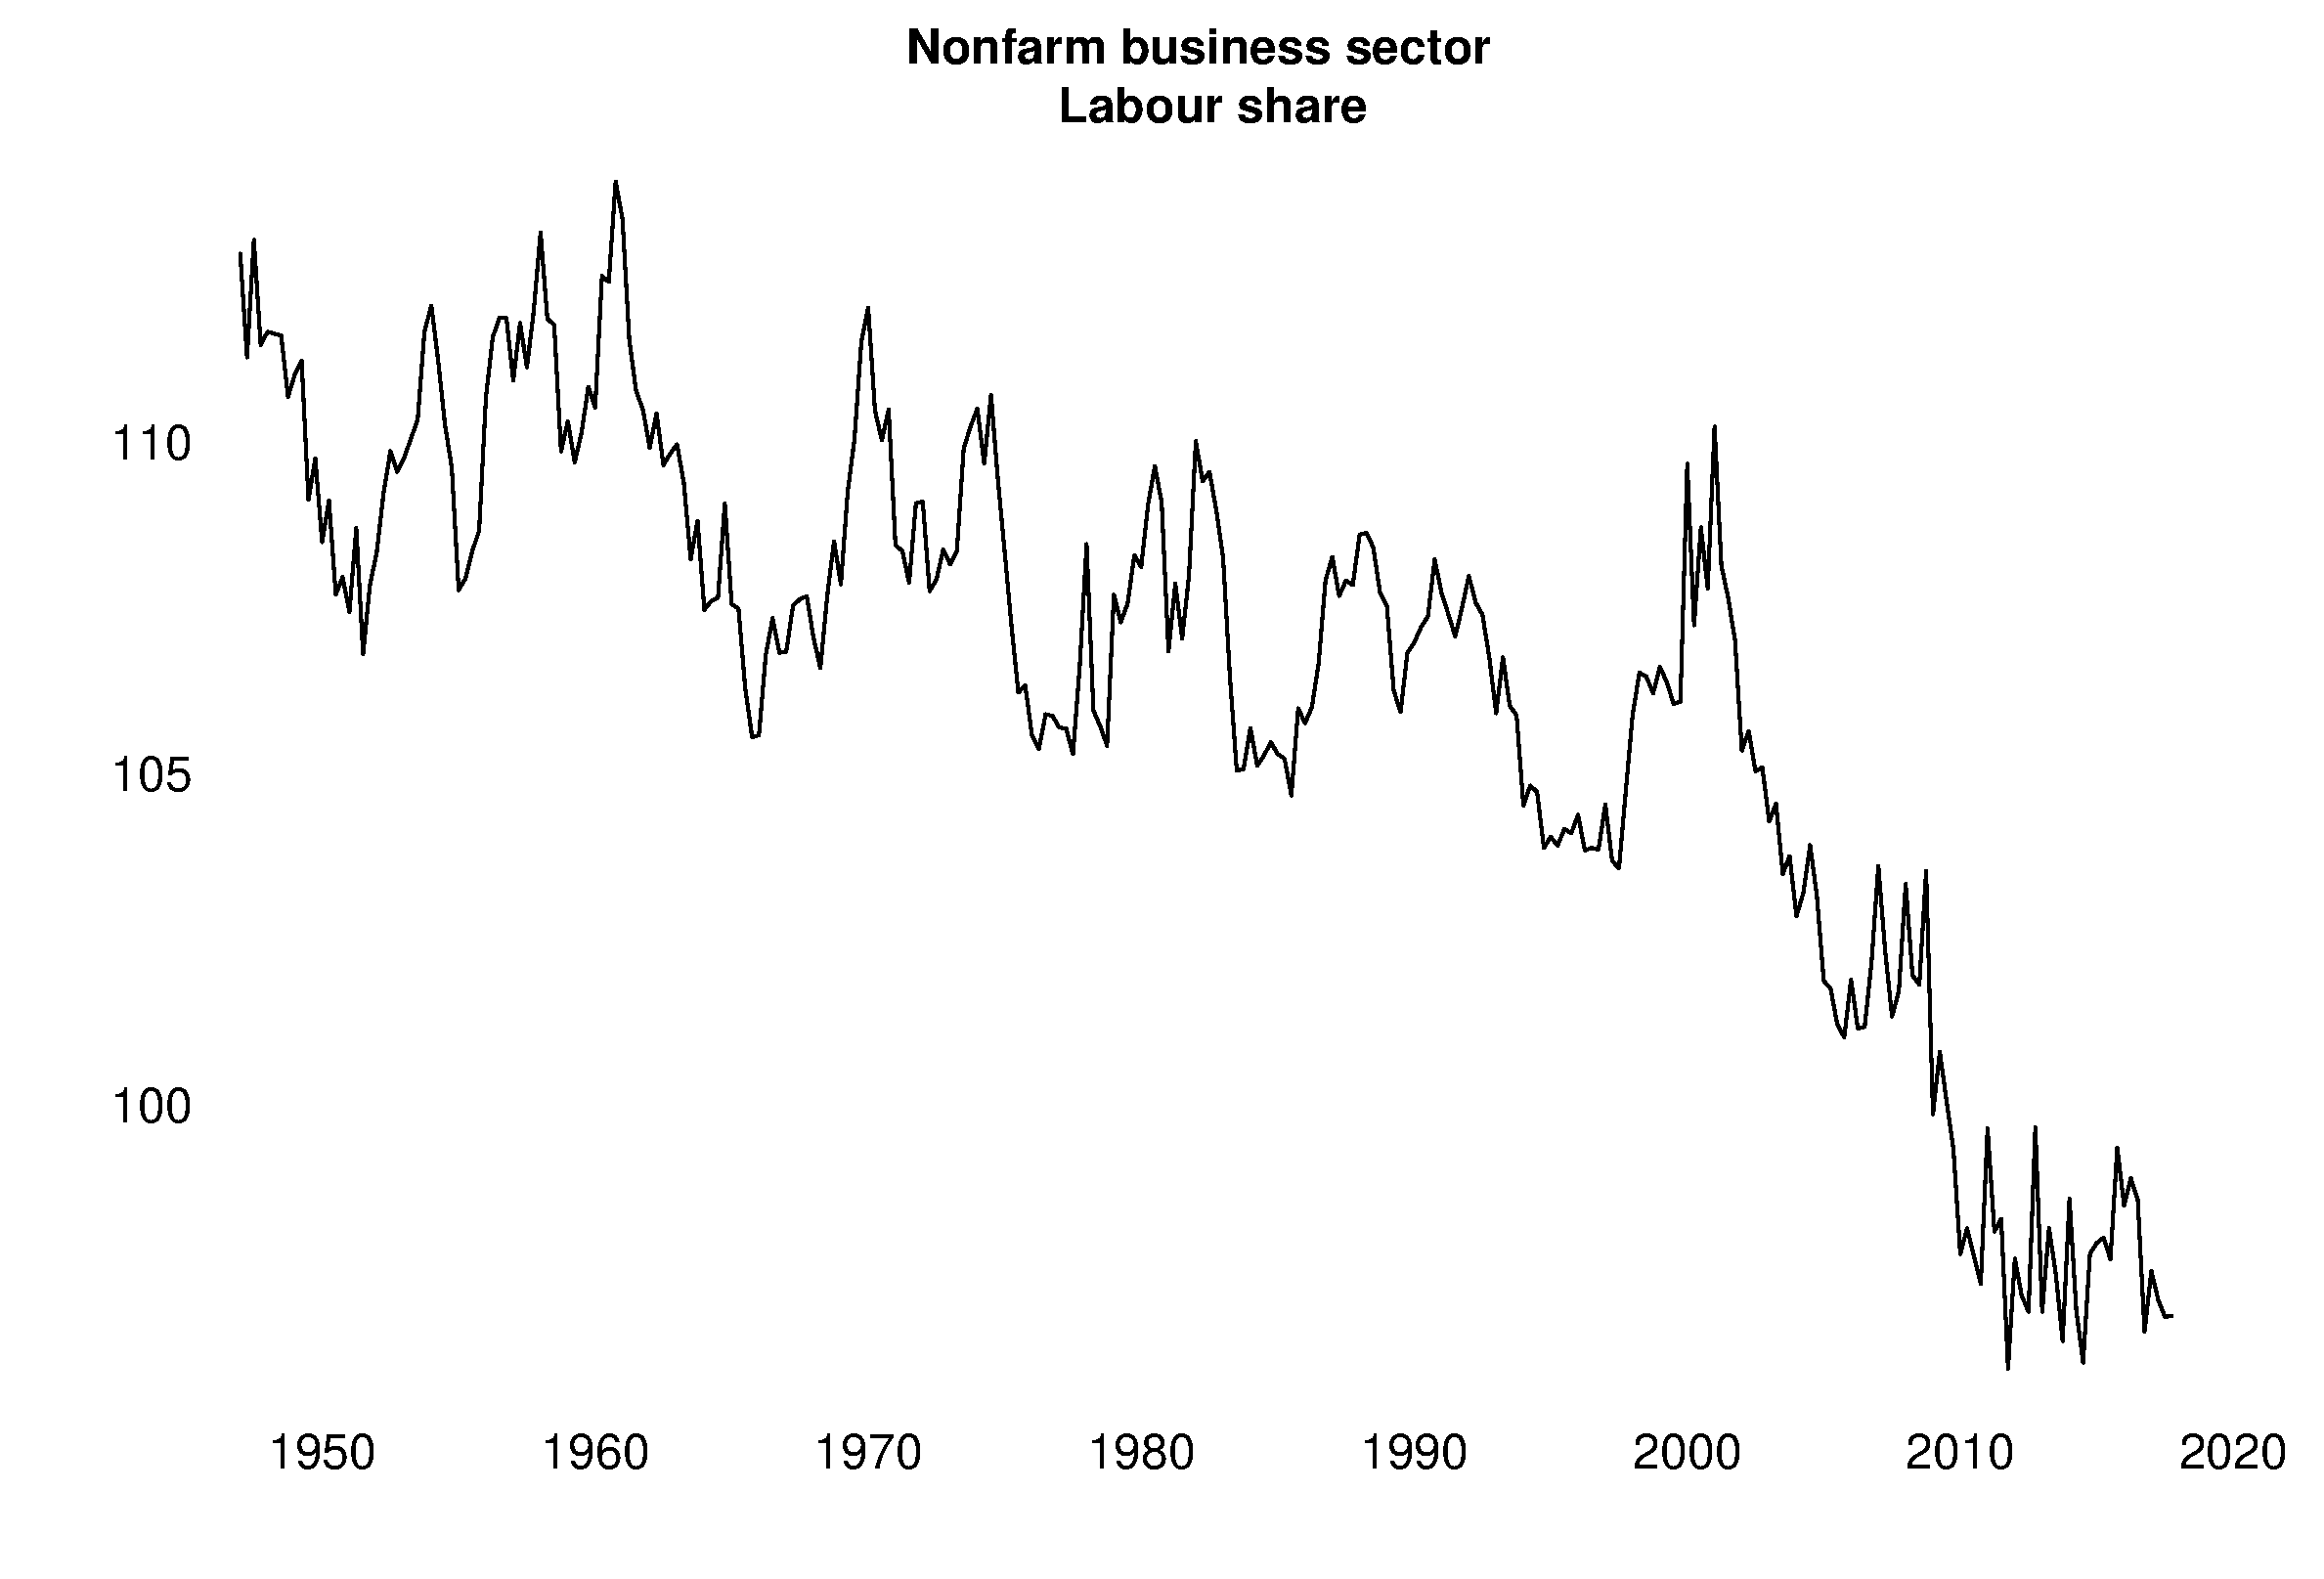
\includegraphics[scale=.25]{labour_share.eps}
  \end{figure}
\end{frame}
%--------------------------------------

%--------------------------------------
\begin{frame}
Some issues
  \begin{itemize}    
    \item Real marginal costs should be procyclical: increase when output is above potential
    \item Labour share is countercyclical
    \item Downward trend in labour share across countries
  \end{itemize}
  \medskip
\textbf{Rudd \& Whelan} (2007) argue that if NKPC works well with labour share this implies that it is completely forward looking
\begin{align}
  \pi_t = \gamma \sum_{k=0}^{\infty} \beta^k \mathbb{}_t s_{t+k}
\end{align}
Can use VAR model to forecast level of $s_{t+k}$ and give a fitted value for the equations above.
\end{frame}
%--------------------------------------

%--------------------------------------
\begin{frame}
 Fit of model not really good (Rudd \& Whelan, 2006); better when including lagged inflation
\begin{align}
  \pi_t = \gamma \sum_{k=0}^{\infty} \beta^k \mathbb{E}_t s_{t+k} + \rho \pi_{t-1}
\end{align}
NKPC's main problem: does not account properly for inflation's dependence on own lags
\end{frame}
%--------------------------------------

%--------------------------------------
\begin{frame}
  Can use a hybrid version
  \begin{align}
    \pi_t = \gamma_f \mathbb{E}_t\pi_{t+1} +\gamma_b \pi_{t-1} + \kappa x_t
  \end{align}
  $x_t$ measures inflationary pressure\\
  Some theoretical weaknesses
  \begin{enumerate}
    \item Rule-of-thumb price-setters: some people set backward-looking prices, other don't (Gali-Gertler, 1999)
    \item Indexation: each period some set optimal prices, others don't; non-optimising price-setters index to past inflation (Christiano et al, 2005)
  \end{enumerate}
\end{frame}
%--------------------------------------


%--------------------------------------
\end{document}
